
\chapter{Introduction}

The Web is an ever growing institution, in all aspects that it covers.
The number of data and functionality providing \textrm{\glspl{webresource}} is growing in the whole spectrum from bigger computing centers down to smaller devices.
Computing centers are growing in size and quantity and they allow for massive amounts of data to be stored and accessed, moreover they also enable the construction and offering of more complex functionality.
At the same time, a quickly increasing number of ever smaller devices also provides more resources to the Web.
Many of them are providing access to the Web itself, granting even more devices access and thus leverage the effect of the growing Web, e.g. mobile phones can act as a hotspot to grant Web access to other devices over \textrm{WiFi}.
A recent trend that can be observed is also all the smart things, which are gaining access to the Web and start to form the \textrm{\gls{webofthings}}.
Today, these smart things can be everything from a temperature sensor to all the electronic devices within a house.
They do not only provide sensor data but they can also be controlled over the Web.
All these different types of services available on the Web make it a heterogeneous collection of data and functionality.
Great efforts are made to turn them into uniformly accessible resources, e.g. the \textrm{\gls{semanticweb}} is a widely supported initiative towards a machine-readable, structured and semantically descripted Web.

Confronted with this rapid growth of the Web, an increasing number of human beings is exposed to it in their daily life, and they get literally flooded with informations and means to retrieve them.
Even though users have access to so much data and functionality in the Web, they often lack the knowledge, necessary time or right approach to weave them together.
It would be of great value for them to automatically get appropriate informations, in the right moment and in a condensed matter that supports them best.
They should be able to automate tedious tasks, e.g. detecting relevant changes in their preferred data resources and react on behalf of such changes.
This requires the identification of and filtering for user-relevant changes, appropriate timing, assembly and processing of additional data and finally the placement of the outcome in the user's preferred context on the Web.

With the many existing services on the Web, users don't want to be bound to specific ones for certain tasks, as it is often the case nowadays.
They want to use the functionality or data of their preferred service, which helps them best to fulfill their needs.
Hence, users should be able to create their own specific but still flexible \textrm{\glspl{webresource}} compositions.
Since the need of users to compose different services has gotten a lot of attention, some of the services on the Web offer ways to spread their data to others, but in a limited way.
For example it is common for social network applications to push user-specific notifications to other social networks, e.g. singing in at a place in \textrm{Foursquare} can also be posted directly to the \textrm{Facebook} timeline.
Because of existing limitations, such as customizability or free choice of receiving service, users still end up mixing data and functionality from different resources on the Web by hand, which often means to execute similar tasks repeatedly by hand.
Moreover the manual reaction on changes is deferred because the changes are not detected in real-time by the user or because the user is not able to react in a timely fashion.
Also if a certain workflow could be split up into several automated sub tasks, it is likely that some parts could be reused for other workflows or even by other people to get similar work done.

Since data and functionality already exist in the Web, the users are theoretically enabled to automate their work to some extent by orchestrating those \textrm{\glspl{webresource}}.
Even though the access to resources gets simpler, the average user is still not capable to fully exploit the Web's full potential.
Another challenge is, that often a lot of effort has to be made, in understanding how the specific resource works, before it can be fully exploited.
There is a lot of research that goes towards an easy to orchestrate the Web, but they are either often complicated to wield themselves, mere data copy tasks or static resource compositions.
Our goal is to enable user-defined resource composition, and still exploiting their full potential by not limiting the set of their functionality.

A big part of the data, that becomes available to the users, is short-lived data that corresponds to state changes, and which can be modeled as events.
In this thesis we introduce an event-driven conceptual model that uses the programmability of the Web and imposes reactivity to it.
We claim the whole Web as our information space, in which we listen for triggered events and in which we execute actions as a result wherever possible.
Such a user-specific reactivity allows a personalization of the Web and a tool to govern its data flood by automating tedious tasks.
It allows users to orchestrate the Web and to tailor reactivity to their needs.
Current \textrm{\gls{webresource}} orchestrations concentrate on data flow rather than on event flow, which are mere copy/paste tasks of data than smart reactivity.
This makes us believe that our event-based conceptual model can overcome certain shortcomings of the existing approaches and provides a step towards the reactive Web.


\begin{figure}[!ht]
  \centering
  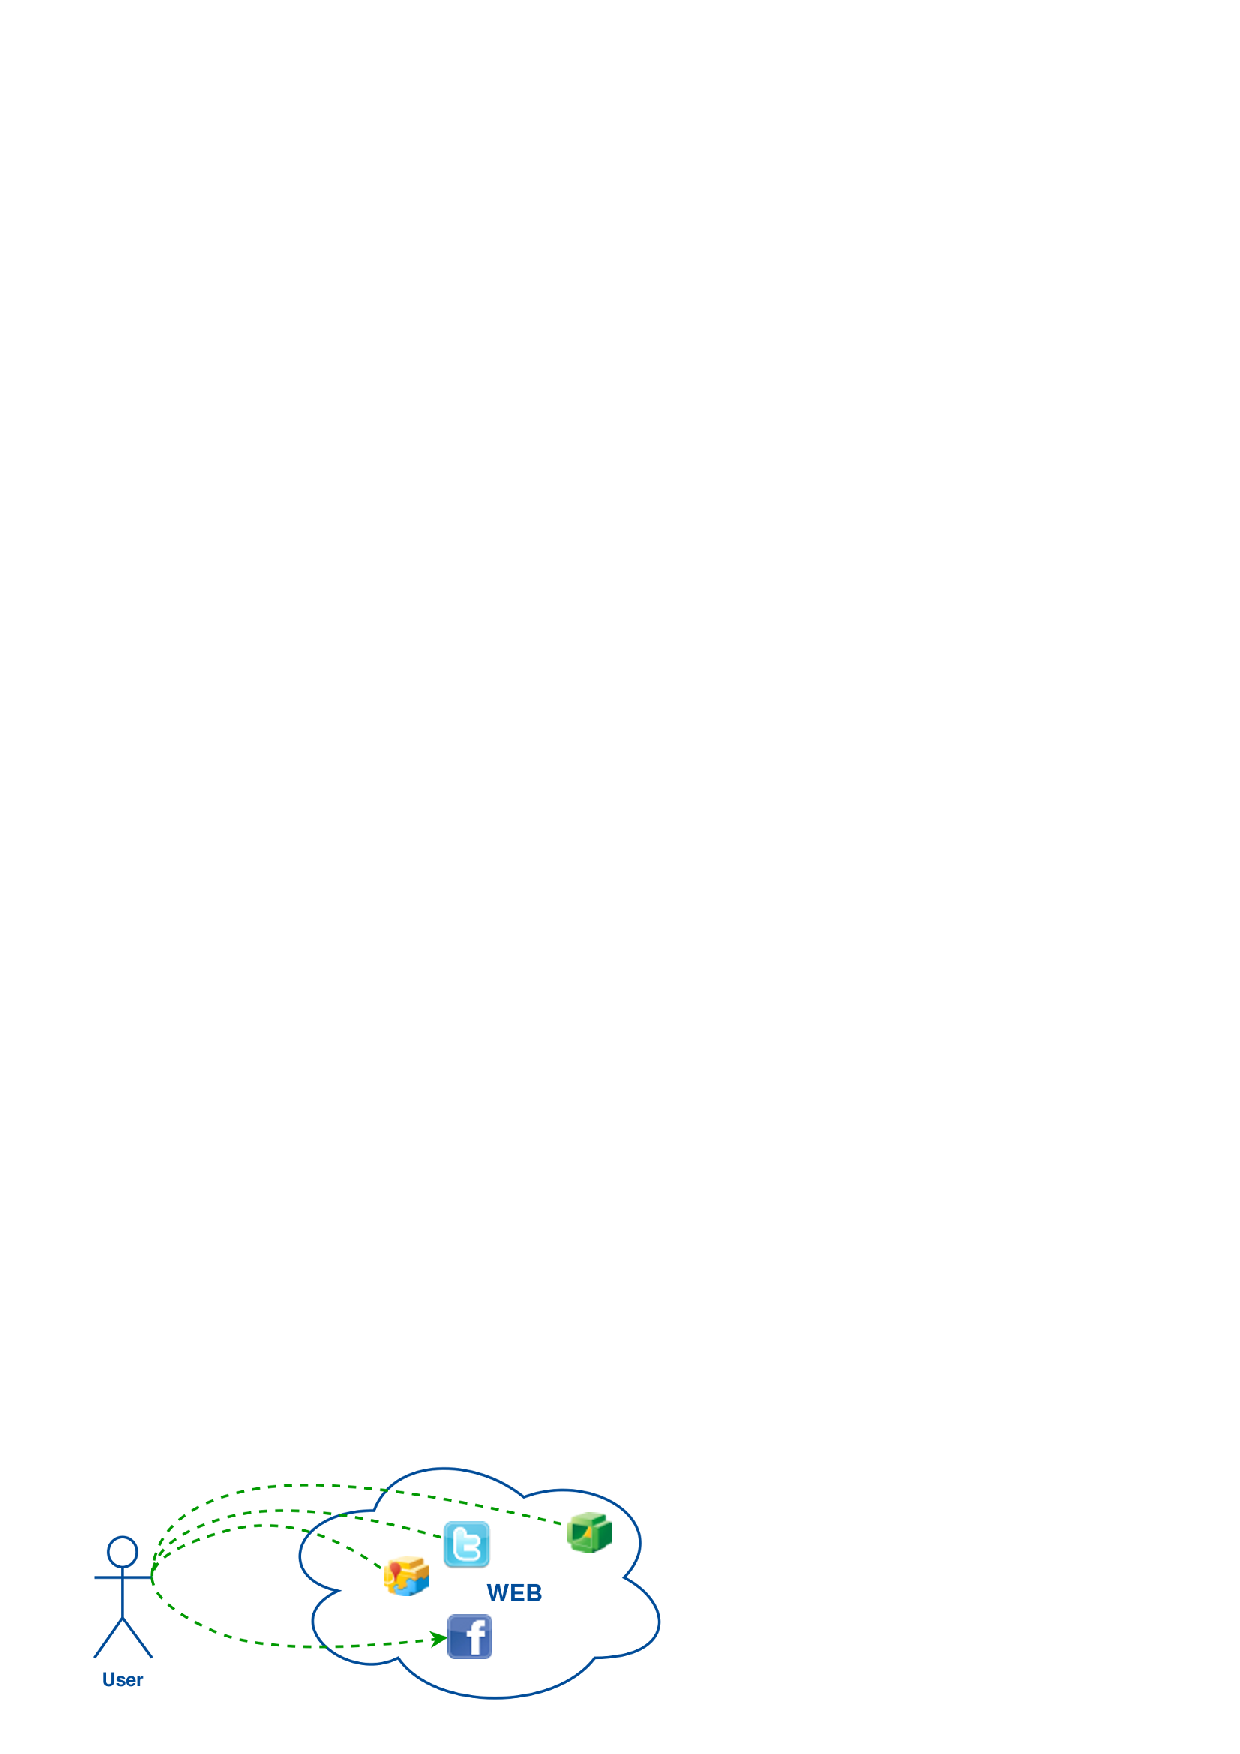
\includegraphics[width=0.7\textwidth]{figures/UsersWeildServicesInTheWeb}
  \caption{Users orchestrate the Web's Data and Functionality}
  \label{fig:UsersWeildServicesInTheWeb}
\end{figure}
% \textit{\small{MAKE NEW ONE! Figure with user orchestrating Web Resources}}
% \textit{\small{ewwww ugly figure....\\
% TODO show more concrete example with aha effect, light bulb. maybe parallel or serial events that turn into a result}}


% \textit{\small{TODO: use the word task or workflow?}}